%%%%%%%%%%%%%%%%%%%%%%%%%%%%%%%%%%%%%%%%%%%%%%%%%%%%%%%%%%%%%%%%%%%%%%%%%%%%%%
%%
%% Dokumentacia k projektu 'Interpret pre jazyk IFJ 2013'
%%
%%
%%%%%%%%%%%%%%%%%%%%%%%%%%%%%%%%%%%%%%%%%%%%%%%%%%%%%%%%%%%%%%%%%%%%%%%%%%%%%%
\documentclass[12pt,a4paper,titlepage,final]{article}

% jazyk
\usepackage[slovak]{babel}
\usepackage[utf8]{inputenc}
% balicky prr odkazy
\usepackage[bookmarksopen,colorlinks,plainpages=false,urlcolor=blue,unicode]{hyperref}
\usepackage{url}
% obrazky
\usepackage[dvipdf]{graphicx}
% velikost stranky
\usepackage[top=3.5cm, left=2.5cm, text={17cm, 24cm}, ignorefoot]{geometry}
\usepackage{caption}
\usepackage{subcaption}


\begin{document}

%%%%%%%%%%%%%%%%%%%%%%%%%%%%%%%%%%%%%%%%%%%%%%%%%%%%%%%%%%%%%%%%%%%%%%%%%%%%%%
% titulní strana

\def\projname{Okruh 4. Výrobný podnik}


\begin{titlepage}

% \vspace*{1cm}
\begin{figure}[!h]
  \centering
  \includegraphics[height=5cm]{doc/logo.eps}
\end{figure}
\center Fakulta Informačních Technologií \\
\center Vysoké Učení Technické v Brně \\

\vfill

\begin{center}
\bigskip
\begin{Huge}
\projname\\
\end{Huge}
\begin{large}
Modelovanie a simulácie\\
\end{large}
\end{center}

\vfill

\begin{center}
\begin{Large}
\today
\end{Large}
\end{center}

\vfill

\begin{flushleft}
\begin{large}
Marek Milkovič (xmilko01)\\
Lukáš Vrabec (xvrabe07) \\
\end{large}
\end{flushleft}
\end{titlepage}

%%%%%%%%%%%%%%%%%%%%%%%%%%%%%%%%%%%%%%%%%%%%%%%%%%%%%%%%%%%%%%%%%%%%%%%%%%%%%%
% obsah
\pagestyle{plain}
\pagenumbering{gobble}
\tableofcontents

%%%%%%%%%%%%%%%%%%%%%%%%%%%%%%%%%%%%%%%%%%%%%%%%%%%%%%%%%%%%%%%%%%%%%%%%%%%%%%
% textova zprava
\newpage
\pagestyle{plain}
\pagenumbering{arabic}
\setcounter{page}{1}

% sekcia 1
%%%%%%%%%%%%%%%%%%%%%%%%%%%%%%%%%%%%%%%%%%%%%%%%%%%%%%%%%%%%%%%%%%%%%%%%%%%%%%
\section{Úvod}
V tejto práci je riešená implementácia modelu(\cite{peringer-slidy} str.7) hypotetického
výrobného podniku na produkciu základných dosiek, ktorá bude použitá pre 
vytvorenie simulačného modelu(\cite{peringer-slidy} str.46) systému(\cite{peringer-slidy} str.7).

Na základe modelu a simulačných experimentov(\cite{peringer-slidy} str.168)
(ďalej len experimenty) bude ukázané chovanie systému (\cite{peringer-slidy} str.24)
výrobného podniku v podmienkach rôzneho vyťaženia(\cite{peringer-slidy} str.139),
pridávania jednotlivých obslužních liniek.
TODO: scim experimentujeme. 

Cieľom experimentov je demonštrovanie možných optimalizácií na zadanom modely. Kon\-kré\-tne
nájdenie optimálnejšej konfigurácie vzhľadom na počet vyrobených
kusov základných dosiek ročne pri čo najmenšej veľkosti a cene výslednej 
výrobnej linky.

Pre spracovanie modelu je nutné naštudovať a pochopiť samotný proces výroby
základnej dosky(ďalej len výroby). Vyhľadať a spracovať informácie týkajúce sa 
technologií ktoré sú použité pri výrobe. Získať technické špecifikácie zariadení,
ktoré sa podieľajú na výrobe. Pri\-spô\-so\-be\-nie modelovaného systému tak,
aby čo najviac odpovedal reálnemu
systému výroby. Následne spracovať tieto údaje, navrhnúť experimenty pré 
vytvorenie optimálnejších riešení výroby. 

%%%%%%%%%%%%%%%%%%%%%%%%%%%%%%%%%%%%%%%%%%%%%%%%%%%%%%%%%%%%%%%%%%%%%%%%%%%%%%
\subsection{Autori a zdroje faktov}
Na projekte sa podieľali študenti VUT FIT Marek Milkovič a Lukáš Vrabec. Informácie
a odborné fakty boli čerpané z internetu, odborných článkov a výročných
správ spoločností GIGA-BYTE Technology Co. Ltd. a ASUSTeK Computer Inc.
Všetky zdroje sú uverejnené na konci tohto dokumentu.

\subsection{Overenie validity modelu}
Validita modelu bola overovaná porovnávaním dát z dostupných zdrojov s výstupmi
simulácie. Pri vytváraní modelu boli čiastočne použité dôverihodné informácie,
pre nedôverihodné alebo nedostupné informácie boli zvolené hypotetické hodnoty,
ktoré približne odpovedajú reálnemu systému. 

% sekcia 2
%%%%%%%%%%%%%%%%%%%%%%%%%%%%%%%%%%%%%%%%%%%%%%%%%%%%%%%%%%%%%%%%%%%%%%%%%%%%%%
\section{Rozbor témy a použitých metód}
%%%%%%%%%%%%%%%%%%%%%%%%%%%%%%%%%%%%%%%%%%%%%%%%%%%%%%%%%%%%%%%%%%%%%%%%%%%%%%
Výrobný podnik spracováva požiadavky na výrobu základných dosiek, ktorý pracuje
v nepretržitej prevádzke. Prvým krokom v procese výroby je vstup dosiek plošných
spojov (\textit{angl.} printable circuit board, ďalej len PCB) do SMT\cite{SMT}
(\textit{angl. surface mount-technology}) liniek, kde dochádza k osadeniu jednotlivých
SMD (\textit{angl. surface-mount device})\cite{SMT} komponent (rezistory, chipset atď.).
SMT linky sa skladajú zo zariadenia pre sieťotlač spájkovacej 
hmoty (\textit{angl. solder paste screen printer})\cite{screen-printer-DEK} kde
dochádza k nanášaniu spájkovacej hmoty na PCB. Tento proces je vykonávaný
2 až 150 mm/sec. Ďalej pokračuje do P\&P (\textit{angl. Pick-and-Place})\cite{smt-PNP}
prístroja ktorý na PCB umiestni SMD komponenty. Rýchlosť umiestnia SMD komponent
na PCB je 0.25 až 0.5 sekundy na čip. Osadené komponenty je nutné upevniť.
K tomuto účelu sa použije pec\cite{reflow-oven} ktorá pri vysokých teplotách upevní komponenty
(spájkovanie pretavením), trvanie približne 5 minút v závisloti na použitom materiále. 

Proces pokračuje kontrolou nanometrových chýb spojov na PCB. Tento proces je 
nazývaný AOI (\textit{angl. automated optical insepction})\cite{AOI}. V prípade výskytu
chýb je PCB nutné manuálne opraviť. Po oprave je nutné AOI zopakovať. Tento
úkon nieje časovo náročny.

Následne je PCB umiestnená na DIP (\textit{angl. Dual in-line package})
linku ktorú predstavuje posuvný pás na ktorom sú manuálne umiesňované 
DIP konektory (DIMM, PCI-Express atď.). DIP konetkory sú upevnené v špeciálnej
peci (spájkovanie vlnou).

Proces výroby základnej dosky je hotový. Vykoná sa viacero manuálnych aj automatizovaných
testov. V prípade chýb je základná doska manuálne opravovaná a sú na nej opakovane vykonané
testy.

Posledným krokom je zabalenie základnej dosky, ktorá je pripravená na distribúciu.

Výrobný podnik môže obsahovať niekoľko SMT, DIP, testovích a baliacích liniek.

\subsection{Popis použitých postupov}
Simulačný model je konzolová aplikácia, naprogramovaná v programovacom jazyku
C++, podľa požiadaviek zadania. Simulačná knižnica SIMLIB/C++\cite{SIMLIB} bola použitá pretože
umožnuje objektovo zapísať model, čím je implementácia jednoduchšia a efektívnejšia.
Z tejto knižnice boli použité aj simulačné nástroje na zber štatistík. Na tvorbu
grafov bol použitý nástroj GNUPLOT\cite{gnuplot}.

\subsection{Popis pôvodu použitých metód}
Bola použitá knižnica SIMLIB/C++, v ktorej sme rozšírili model zariádení a 
skladov o identifikáciu v ktorej výrobnej linke sa nachádza.

% sekcia 3
%%%%%%%%%%%%%%%%%%%%%%%%%%%%%%%%%%%%%%%%%%%%%%%%%%%%%%%%%%%%%%%%%%%%%%%%%%%%%%
\section{Koncepcia modelu}
%%%%%%%%%%%%%%%%%%%%%%%%%%%%%%%%%%%%%%%%%%%%%%%%%%%%%%%%%%%%%%%%%%%%%%%%%%%%%%

Podľa dostupných informáčních zdrojov sa predpokladá ročná výroba 7 miliónov
základných dosiek na továreň, čo je približne 21 miliónov základných dosiek
na spoločnosť\cite{gigabyte-sprava}. Z toho dôvodu je nutné vytvoriť požiadavku na 19179 kusov deňne.
PCB sa radia do spoločnej fronty pred vstupom do SMT liniek. Zvolená je tá SMT
linka na ktorej sa náchádza volné zariadenie pre sieťotlač spájkovacej hmoty.
Predpokladáme rovnomerné trvanie sieťotlače 30 až 45 sekúnd pri nastavení sieťotlače
na 10mm/sec a rozmeroch PCB 305x244 mm (ATX model)\cite{ATX}.

PCB sa ďalej radia do fronty P\&P zariadenia v SMT linke v ktorej sa nachádzajú.
Predpoklad je, že P\&P zariadenie osadí čipy rýchlosťou 0.15 sekundy na čip, pričom
sa predpokladajú hypotetické základné dosky obsahujúce 240 až 480 SMD komponent
z dôvodu nedostatku informácií. Tento proces bude trvať rovnomerne 36 až 72 sekúnd.
PCB sa pohybujú po výrobnej linke za sebou cez pec, tento prechod trvá 5 minút.

Ďalej je zahájený proces AOI zariadení s frontov ktorého trvanie je rovnomerne 10 až 14 sekúnd, v 
prípade že nastane chyba s pravedepodobnosťou 1\% je doska opravovaná. Dĺžka
opravy je daná exponencionálnym rozložením so stredom 6 minuty. Opravené PCB
ktoré musia znova podstúpiť AOI majú vyššiu prioritu ako PCB vstupujúce do AOI 
po prvý krát.

Pri procese prechodu z SMT linky na DIP linku, je vybraná prvá DIP linka s dostupnou
kapacitou, v prípade plného obsadenia DIP liniek je vybraná tá s najkratšou
frontou. Neskôr dochádza k osadzovaniu DIP konetkorov na výrobnej linke
ktorá predstavuje posuvný pás a následne musí základná doska prejsť ďalšou
pecou. Nakoľko je tento proces vykonávaný na jednom posuvnom páse spojenie týchto
procesov nijak neovplivní výsledky modelu. Celý tento proces trvá 2 minuty.

Pri prechode z DIP liniek na testovacie linky je použitý rovnáky mechanizmus
výberu linky ako pri prechode z SMT liniek na DIP linky. V testovacej fáze 
dochádza k manuálnym a automatizovaným testom. Dĺžka testovania je daná 
exponencionálnym rozložením so stredom 2 minuty, pričom v 1\% prípadov dochádza
k potrebe dosku opraviť, dĺžka opravy je daná exponencionálnym rozložením so
stredom 3 minuty. Opravené zákldné dosky musia podstúpiť testovanie znova, pričom
majú vyššiu prioritu.

Nasleduje prechod základných dosiek na baliace linky. Mechanizmus prechodu je
rovnaký ako v prípade prechodu z DIP liniek na testovacie linky. Balenie trvá 
rovnomerne 40 až 60 sekúnd.

V modely sa nepredpokladá s možnou poruchou na zariadeniach z dôvodu nízkej
poruchovosti.

\subsection{Návrh konceptuálneho modelu}
Požiadavok na výrobu základnej dosky vstupuje do systému kde sa zaraďuje do fronty
SMT liniek. Postupuje cez solder paste screen printer, P\&P a AOI, ktoré 
sú modelované ako zariadenia. Presúva sa na DIP linku, následne na testovaciu
a baliacu linku ktoré sú modelované ako sklad. Následne proces predstavujúci
hotovú základnú dosku opúšta systém.

\subsection{Formy konceptuálneho modelu}
Linky sú znazornené pomocou samotných petriho sietí(\cite{peringer-slidy} str. 123),
nakoľko prechody medzi linkami nebolo možné namodelovať a jednotlivých liniek 
može byť v systéme niekoľko. Jednotlivé petriho siete sa napájajú na prázdne
miesto na konci každej siete. 

\begin{figure}[!h]
  \centering
  \includegraphics[width=17cm]{doc/smt.png}
  \caption{SMT linka}
\end{figure}

\begin{figure}[!h]
  \centering
  \includegraphics[width=10cm]{doc/dip.png}
  \caption{DIP linka}
\end{figure}

\begin{figure}[!h]
  \centering
  \includegraphics[width=14cm]{doc/tst.png}
  \caption{Testovacia linka}
\end{figure}

\begin{figure}[!h]
  \centering
  \includegraphics[width=10cm]{doc/pkg.png}
  \caption{Baliaca linka}
\end{figure}

% sekcia 4
%%%%%%%%%%%%%%%%%%%%%%%%%%%%%%%%%%%%%%%%%%%%%%%%%%%%%%%%%%%%%%%%%%%%%%%%%%%%%%
\section{Architektúra simulačného modelu}
%%%%%%%%%%%%%%%%%%%%%%%%%%%%%%%%%%%%%%%%%%%%%%%%%%%%%%%%%%%%%%%%%%%%%%%%%%%%%%
V implementácií boli použité triedy knižnice SIMLIB/C++. Ako generátor požiadavkov
na výrobu bola použitá trieda \texttt{Event}, tento generátor je aktivovaný počas simulácie
v čase 0, následne je spušťaný každých 24 hodín. Generátor vytvára požiadavky typu
\texttt{Board}, ktoré dedia triedu \texttt{Process}.

Doba simulácie je nastavená na 1 rok. Časová jednotka použitá v simulácií je 
sekunda.

\subsection{Mapovanie abstraktného modelu do simulačného modelu}
Všetky zariadenia na výrobných linkách sú odvodené od triedy \texttt{Machine}
a všetky sklady od triedy \texttt{Line}. Obe tieto triedy umožnujú identifikovať
na ktorých výrobných linkách sa nachádzajú. Generátor požiadavkov na výrobu základných
dosiek je implementovaný v triede \texttt{Generator}. Trieda \texttt{Board} predstavuje
základnú dosku od počiatku výrobného procesu až po jej zabalenie. 

\subsection{Použitie programu}
Simulácia sa kompiluje pomocou príkazu \texttt{\$ make}. Sputenie experimentov
je prevádzané pomocou príkazu \texttt{\$ make run}. Parametre umožnujúce modifikovať
simulačný model sú nasledovné.

\begin{table}[h]
\centering
\begin{tabular}{|l|l|}
\hline
\multicolumn{1}{|c|}{\textbf{Parameter}} & \multicolumn{1}{c|}{\textbf{Popis}}  \\ \hline
\texttt{--smt N}    & Pri sumlácií bude použitých N SMT liniek.                          \\ \hline
\texttt{--dip N}    & Pri sumlácií bude použitých N DIP liniek.                          \\ \hline
\texttt{--tst N}    & Pri sumlácií bude použitých N testovacích liniek.                  \\ \hline
\texttt{--pkg N}    & Pri sumlácií bude použitých N baliacich liniek.                    \\ \hline
\texttt{--req N}    & Bude vygenerovaných N požiadavkov za deň.                          \\ \hline
\texttt{--pnp N M}  & Trvanie výroby na P\&P stroji bude rovnomerne N až M sekúnd.       \\ \hline
\texttt{--out FILE} & Výstup bude presmerovaný do súboru FILE.                           \\ \hline
\texttt{--err N M}  & Chyba na AOI nastane v N\% prípadov, pri testovaní v M\% prípadov. \\ \hline
\end{tabular}
\end{table}


% sekcia 5
%%%%%%%%%%%%%%%%%%%%%%%%%%%%%%%%%%%%%%%%%%%%%%%%%%%%%%%%%%%%%%%%%%%%%%%%%%%%%%
\section{Simulačné experimenty a ich priebeh}
%%%%%%%%%%%%%%%%%%%%%%%%%%%%%%%%%%%%%%%%%%%%%%%%%%%%%%%%%%%%%%%%%%%%%%%%%%%%%%
Cieľom experimentov s reprezentáciou simulačného modelu bolo zistiť, vyťaženie
liniek počas výrobného procesu v rámci jedného dňa a schopnosť produkcie 7 miliónov
dosiek za rok\cite{gigabyte-sprava}.

Vytvorenie simulačného modelu bolo nutné, nakoľko hypotetický model je príliš
zložitý na popis a riešenie pomocou analitických rovníc.

\subsection{Postup experimentovania}
Z dôvodu podania čo najlepšie pozorovateľných výsledkov experimentov, bol 
generátor pseudonáhodných čísel(\cite{peringer-slidy} str. 97) inicilizovaný hodnotou(\textit{angl. seed})
aktuálného času. Priebeh experimentov prebiehal tak, že boli modifikované 
vlastnosti jednotlivých prvkov sýstému alebo boli pridávané/odoberané výrobné
linky.

\subsection{Popis experimentov}
Prvý experiment vykonávame so základnou konfigurácou simulačného modelu, z toho 
dôvodu sa nazýva referenčny experiment. 

Všetky ďalsie experimenty budú výchádzať z referenčného. Z výsledkov referenčného
experimentu budu vyvodené závery, na základe ktorých budu vykonávané ostané experimenty.
Dôraz bude kladený na zmenu parametrov, ktoré sú nachýlené k zmenám vlastností
systému.

\subsubsection{Referenčný experiment}
Východiskovým experiment pre porovnávanie s ďalšími experimentami.
Experiment bol spustený so základnými parametrami. Na základe nižšie uvedených histogramoch
je možné vidiet počet vyrobených dosiek v priebehu dňa, dobu 
výroby základnej dosky (Obr. 5). Ďalej je možné vidiet priemernú dĺžku
fronty u P\&P zariadení (Obr. 6). Zvyšné histogramy zobrazujú priemernú a maximálnu
kapacitu na linkách: SMT (Obr. 7), DIP (Obr. 8), testovacích (Obr. 9) a baliacich (Obr. 10).

\begin{verbatim}
  Vyrobených základných dosiek: 7 000 335 kusov
\end{verbatim}

\begin{figure}[ht]
  \centering
  \begin{minipage}{0.45\linewidth}
  \centering
  \includegraphics[width=8cm]{doc/1_hist1.eps}
  \caption{počet dosiek vyrobených za deň}
  \end{minipage}
  \quad
  \begin{minipage}{0.45\linewidth}
    \centering
    \includegraphics[width=8cm]{doc/1_hist2.eps}
    \caption{doba výroby základnej dosky}
  \end{minipage}
\end{figure}

\begin{figure}[ht]
  \centering
  \begin{minipage}{0.45\linewidth}
  \centering
  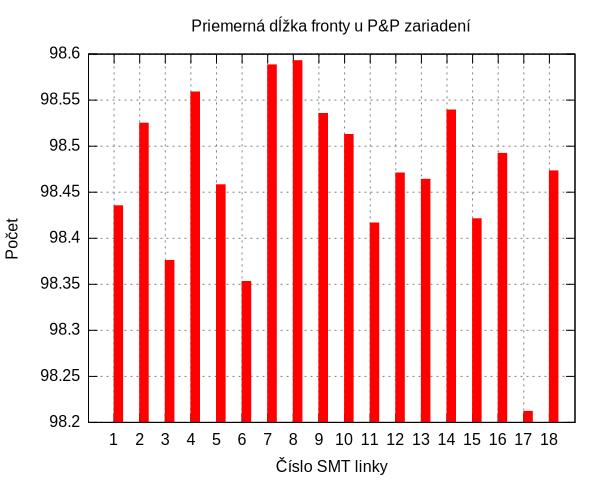
\includegraphics[width=8cm]{doc/1_hist3.eps}
  \caption{priemerná dĺžka fronty u P\&P}
  \end{minipage}
  \quad
  \begin{minipage}{0.45\linewidth}
    \centering
    \includegraphics[width=8cm]{doc/1_hist4.eps}
    \caption{priemerná a maximalna kap. na DIP}
  \end{minipage}
\end{figure}

\newpage

\begin{figure}[ht]
  \centering
  \begin{minipage}{0.45\linewidth}
  \centering
  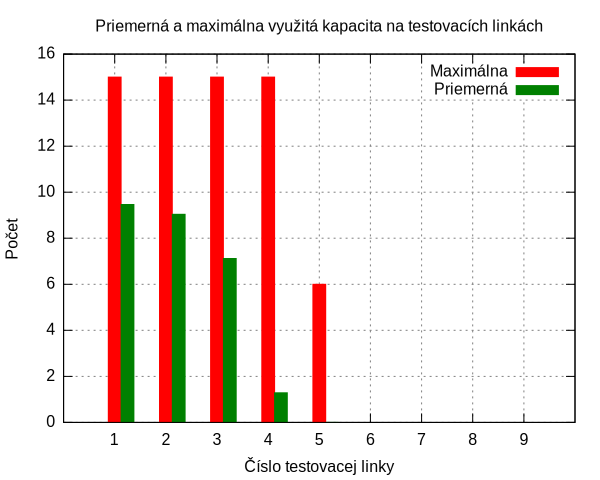
\includegraphics[width=8cm]{doc/1_hist5.eps}
  \caption{priemerná a maximalna kap. na TST}
  \end{minipage}
  \quad
  \begin{minipage}{0.45\linewidth}
    \centering
    \includegraphics[width=8cm]{doc/1_hist6.eps}
    \caption{priemerná a maximalna kap. na PKG}
  \end{minipage}
\end{figure}

Z prvého histogramu je vidieť že výrobný podnik pracuje v čase od 00:00 do 16:00 hod.
V čase 16:00 až 24:00 výrobná linka čaká na prijatie novej požiadavky, čím nieje 
využitá celá jeho schopnosť produkovať základné dosky. Podľa druhého histogramu,
je vidieť že niektoré dosky sú v výrobnom procese 4 až 6 hod, čo znamená že výrobný
proces je v niektorej jeho časti výrazne spomalovaný. K spomalovaniu dochádza 
vo fronte u zariadenia P\&P[link hist.], ktoré je najpomalšie z celej SMT linky.
Zo zvýšních histogramov je vidieť že spomalenie následne spôsobuje že DIP, baliacie aj
testovacie linky sú využité len z časti.

\newpage

\subsubsection{Zrýchlenie P\&P zariadení}
Pri druhom experimente bol kladený dôraz na zrýchlenie P\&P zariadenia 
pričom obsluha dosky trvala rovnomerne 25 až 40 sekúnd, čo 
znížilo veľkosť P\&P front v systéme. V tomto prípade prišlo k veľmi
výraznému zníženiu obsluhy oproti referenčnému experimentu. V nižšie uvedených 
histogramoch možne vidieť lepšie využitie kapacity pri DIP, testovacích a baliacích
linkách, avšak stále niesú využité naplno. 

\begin{verbatim}
  Vyrobených základných dosiek: 7 000 335 kusov
\end{verbatim}

\begin{figure}[!h]
  \centering
  \begin{minipage}{0.45\linewidth}
  \centering
  \includegraphics[width=8cm]{doc/2_hist1.eps}
  \caption{počet dosiek vyrobených za deň}
  \end{minipage}
  \quad
  \begin{minipage}{0.45\linewidth}
    \centering
    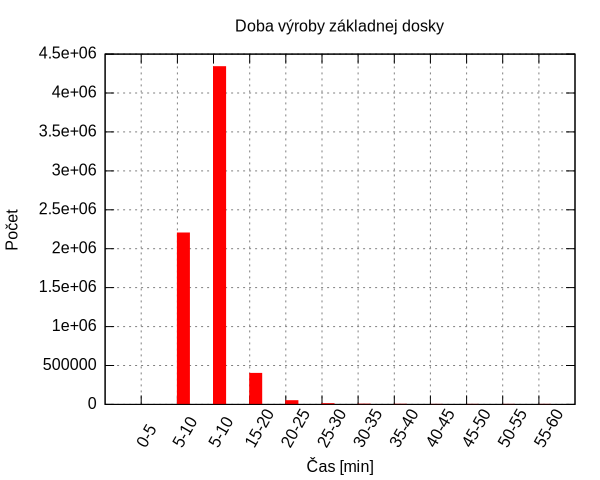
\includegraphics[width=8cm]{doc/2_hist2.eps}
    \caption{doba výroby základnej dosky za min.}
  \end{minipage}
\end{figure}

\begin{figure}[!h]
  \centering
  \begin{minipage}{0.45\linewidth}
  \centering
  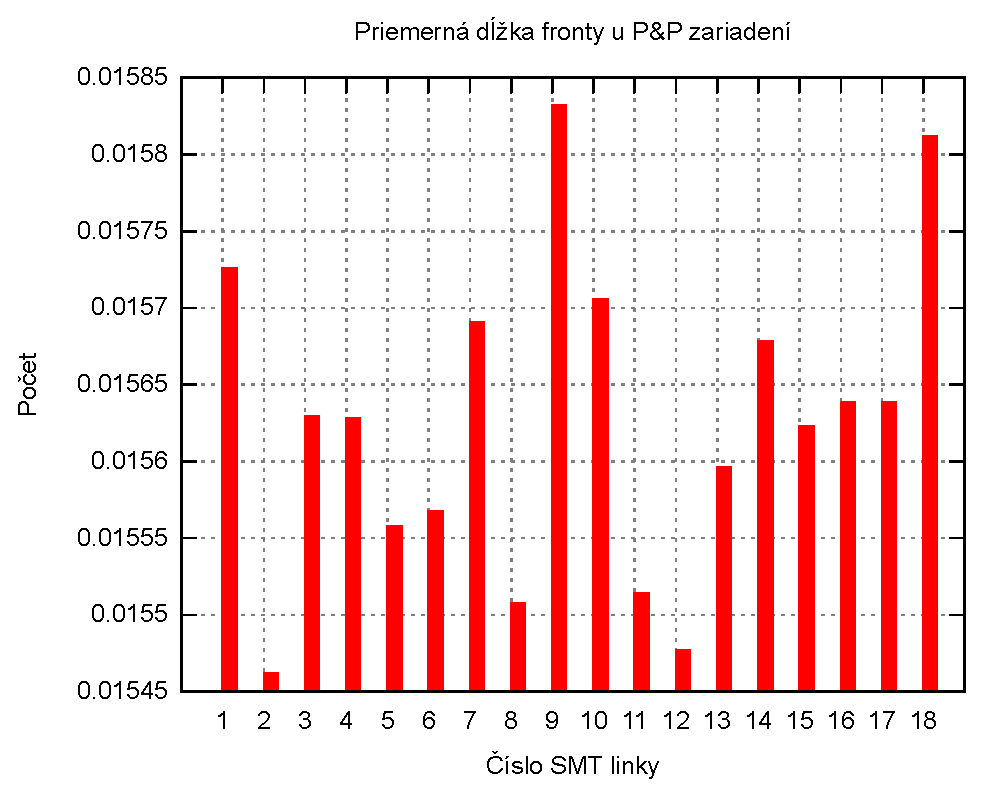
\includegraphics[width=8cm]{doc/2_hist3.eps}
  \caption{priemerná dĺžka fronty u P\&P}
  \end{minipage}
  \quad
  \begin{minipage}{0.45\linewidth}
    \centering
    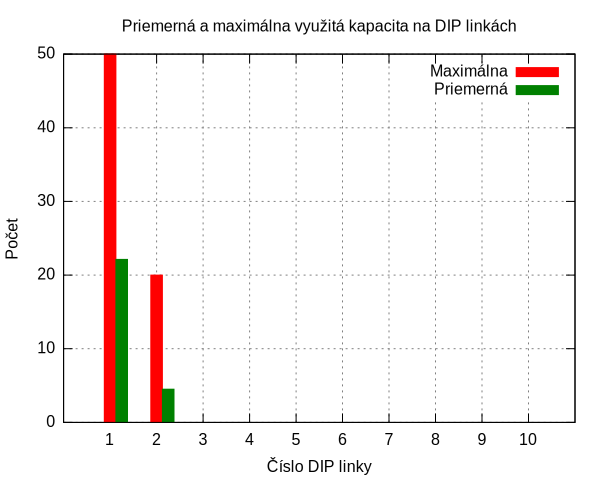
\includegraphics[width=8cm]{doc/2_hist4.eps}
    \caption{priemerná a maximalna kap. na DIP}
  \end{minipage}
\end{figure}

\begin{figure}[!h]
  \centering
  \begin{minipage}{0.45\linewidth}
  \centering
  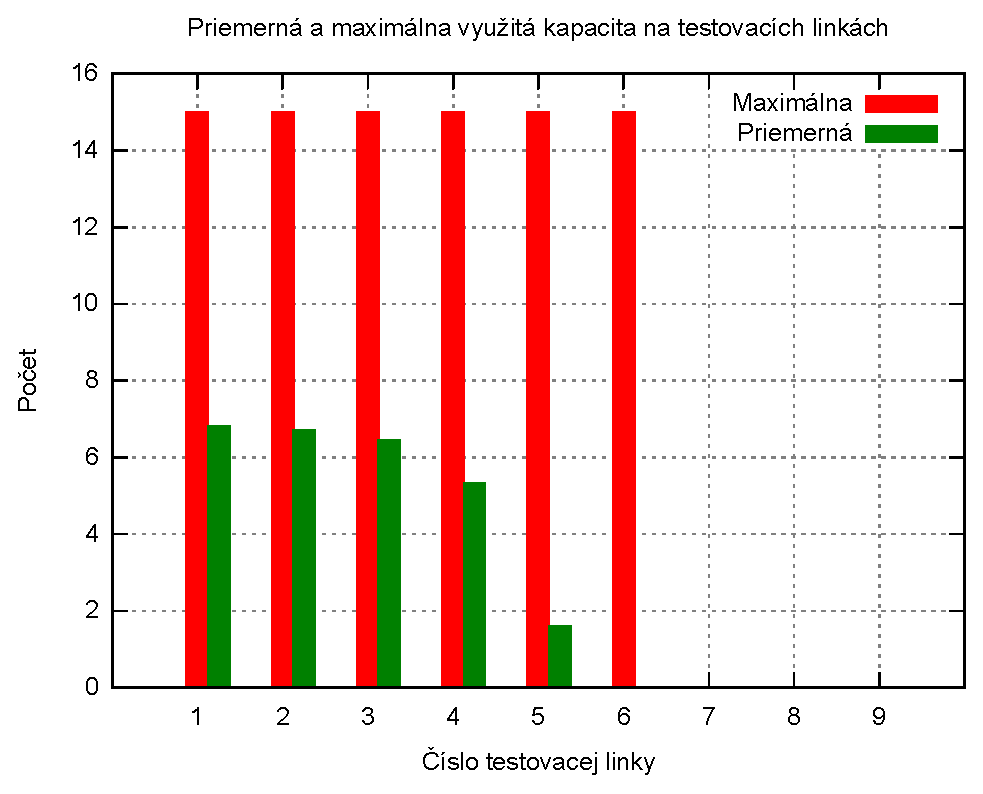
\includegraphics[width=8cm]{doc/2_hist5.eps}
  \caption{priemerná a maximalna kap. na TST}
  \end{minipage}
  \quad
  \begin{minipage}{0.45\linewidth}
    \centering
    \includegraphics[width=8cm]{doc/2_hist6.eps}
    \caption{priemerná a maximalna kap. na PKG}
  \end{minipage}
\end{figure}

\newpage

\subsubsection{Zvýšená produkcia}

\begin{verbatim}
  Vyrobených základných dosiek: 12 775 00 kusov
\end{verbatim}

\begin{figure}[!h]
  \centering
  \begin{minipage}{0.45\linewidth}
  \centering
  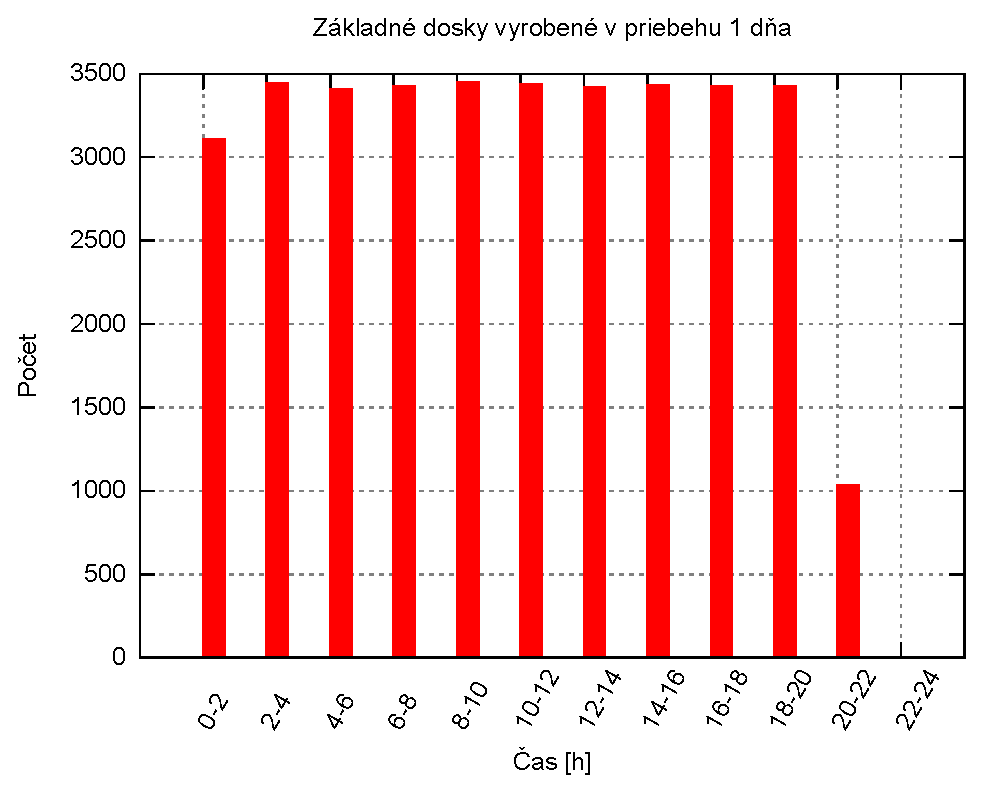
\includegraphics[width=8cm]{doc/3_hist1.eps}
  \caption{počet dosiek vyrobených za deň}
  \end{minipage}
  \quad
  \begin{minipage}{0.45\linewidth}
    \centering
    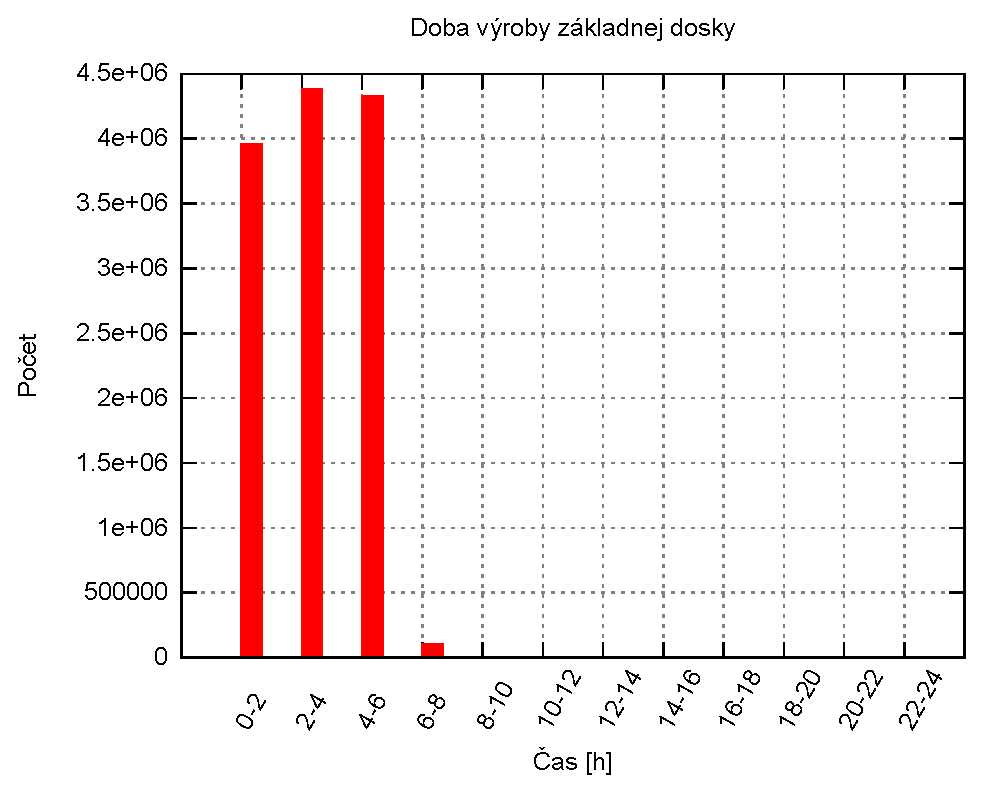
\includegraphics[width=8cm]{doc/3_hist2.eps}
    \caption{doba výroby základnej dosky za min.}
  \end{minipage}
\end{figure}

\begin{figure}[!h]
  \centering
  \begin{minipage}{0.45\linewidth}
  \centering
  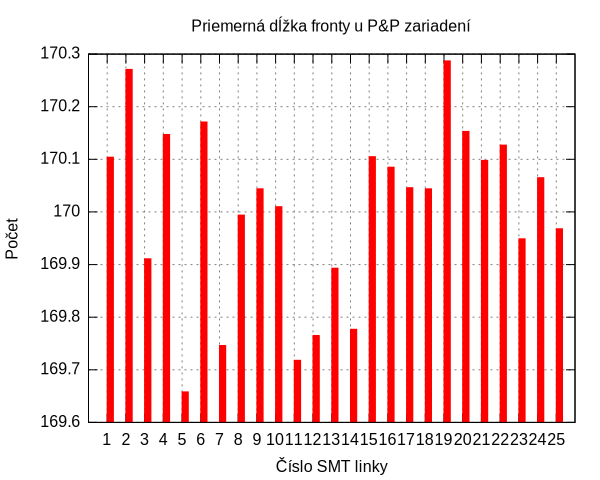
\includegraphics[width=8cm]{doc/3_hist3.eps}
  \caption{priemerná dĺžka fronty u P\&P}
  \end{minipage}
  \quad
  \begin{minipage}{0.45\linewidth}
    \centering
    \includegraphics[width=8cm]{doc/3_hist4.eps}
    \caption{priemerná a maximalna kap. na DIP}
  \end{minipage}
\end{figure}

\begin{figure}[!h]
  \centering
  \begin{minipage}{0.45\linewidth}
  \centering
  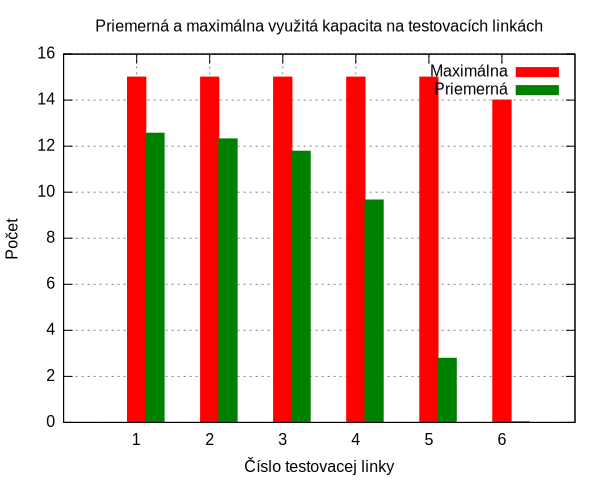
\includegraphics[width=8cm]{doc/3_hist5.eps}
  \caption{priemerná a maximalna kap. na TST}
  \end{minipage}
  \quad
  \begin{minipage}{0.45\linewidth}
    \centering
    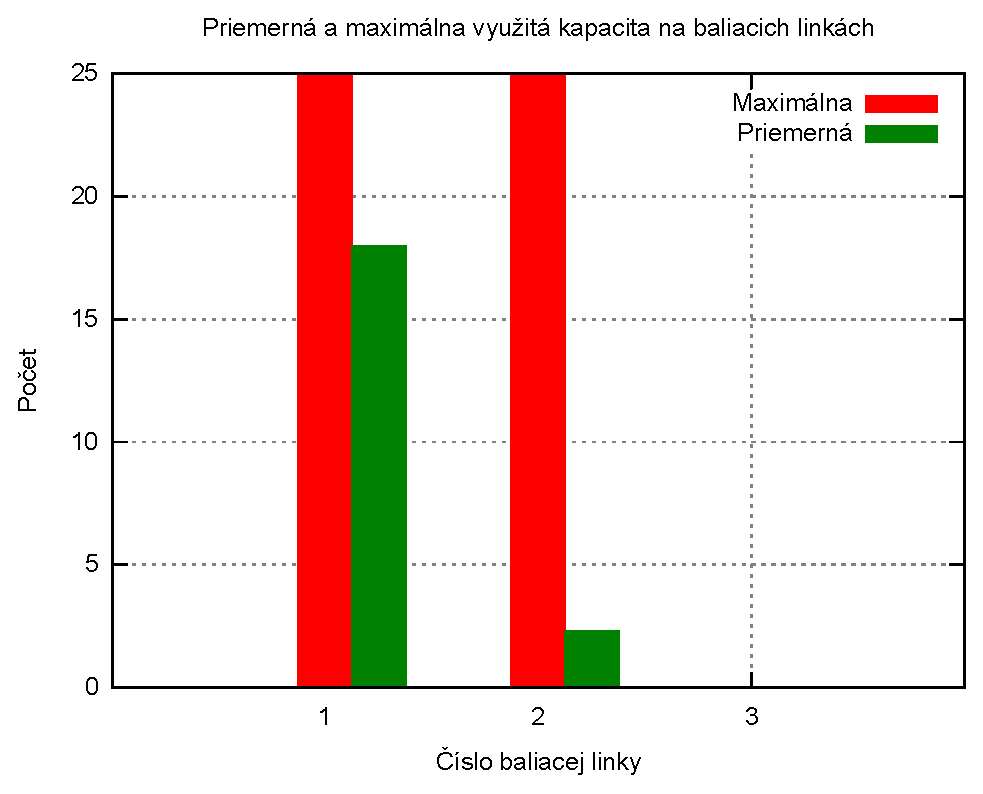
\includegraphics[width=8cm]{doc/3_hist6.eps}
    \caption{priemerná a maximalna kap. na PKG}
  \end{minipage}
\end{figure}

\newpage

% sekcia 6
%%%%%%%%%%%%%%%%%%%%%%%%%%%%%%%%%%%%%%%%%%%%%%%%%%%%%%%%%%%%%%%%%%%%%%%%%%%%%%
\section{Zhrnutie simulačných experimentov a záver}
%%%%%%%%%%%%%%%%%%%%%%%%%%%%%%%%%%%%%%%%%%%%%%%%%%%%%%%%%%%%%%%%%%%%%%%%%%%%%%

\begin{thebibliography}{9}

\bibitem{peringer-slidy} 
PERINGER, P.: Modelování a simulace, september 2014, (VUT FIT v Brne), IMS - slajdy z
prednášok.

\bibitem{screen-printer-DEK} 
DEK Printing Machines Limited. [online], 2000.
\\\texttt{URL <http://www.pcbtechnology.pl/wp-content/uploads/2014/02/dek-infinity-spec.pdf>}

\bibitem{smt-PNP} 
FUJI MACHINE MFG. CO., LTD. [online], 2013.
\\\texttt{URL <https://smt.fuji.co.jp/e/products/mounter/detail.php?id=8>}

\bibitem{reflow-oven} 
IXYS Corporation. [online], 2006.
\\\texttt{URL <http://www.ixys.com/Documents/AppNotes/IXAN0059.pdf>}

\bibitem{AOI} 
Nordson YESTECH. [online].
\\\texttt{URL <http://www.nordson.com/en-us/divisions/yestech/Literature/NYT-FXSeries\_DS\%28L\%29.pdf>}

\bibitem{gigabyte-sprava} 
GIGA-BYTE Technology Co., Ltd. [online], 2013.
\\\texttt{URL <http://www.gigabyte.com/fileupload/sitemap/36/images/AnnualReportEng-2013.pdf>}

\bibitem{asus-sprava} 
ASUSTeK Computer Inc. [online], 2013.
\\\texttt{URL <http://www.annualreportowl.com/Asus/2013/Annual\%20Report>}

\bibitem{gnuplot} 
WILLIAMS, T.; KELLEY, C.; LANG, R.: Gnuplot. [online], Naposledy upravené november 2014.
\\\texttt{URL <http://www.gnuplot.info>}

\bibitem{SMT} 
WILLIAMS, P.: SURFACE MOUNT COUNCIL. [online], august 1999.
\\\texttt{URL <http://www.ipc.org/4.0_Knowledge/4.1_Standards/smcstatus.pdf>}

\bibitem{SIMLIB} 
PERINGER, P.: SIMLIB/C++. [online], Naposledy upravené 27. 03. 2014.
\\\texttt{URL <http://www.fit.vutbr.cz/~peringer/SIMLIB/>}

\bibitem{ATX} 
Intel Corporation: ATX Specification. [online], 2004.
\\\texttt{URL <http://www.formfactors.org/developer/specs/atx2_2.pdf>}

\end{thebibliography}

\end{document}
